%------------------------------------------
%	$Id: GMT_Appendix_P.tex,v 1.13 2008-02-29 03:30:34 remko Exp $
%
%	The GMT Documentation Project
%	Copyright 2000-2008.
%	Paul Wessel and Walter H. F. Smith
%------------------------------------------
%

\chapter{Special Operations}
\label{app:P}
\thispagestyle{headings}

\section{Running \gmt\ in \emph{isolation mode}}
\label{sec:isolationmode}
\index{Isolation mode|(}
In Chapter~\ref{ch:4} it is described how \GMT\ creates several (temporary) files to communicate between the different commands that make up the script that finally creates a plot. Among those files are:
\begin{description}
\item[\filename{.gmtdefaults4}.] This file covers about 100 different settings that influence the layout of your plot, from font sizes to tick lengths and date formats (See Section~\ref{sec:gmtdefaults}). Those settings can be altered by editing the file, or by running the \GMTprog{gmtset} command. A problem may arise when those settings are changed half-way the script: the next time you run the script it will start with the modified settings and hence might alter your scripts results. It is therefore often necessary to revert to the original \filename{.gmtdefaults4} file. \emph{Isolation mode} avoids that issue.
\item[\filename{.gmtcommands4}.] This file is created to communicate the command line history from one command to the next (Section~\ref{sec:gmtcommands}) so that shorthands like \Opt{R} or \Opt{J} can be used once it has been set in a previous \GMT\ command.
The existence of this file makes if impossible to run two \GMT\ scripts simultaneously in the same directory, since those \filename{.gmtcommand4} files may clash (contain different histories) and adversely affect the results of both scripts.
\item[\filename{.gmt\_bb\_info}.] This file contains the information about the BoundingBox (Section~\ref{sec:eps}) of the \PS\ output. This information too has to be transferred from one \GMT\ command to the next in a script. Again, running two commands simultaneously in the same directory may have disastrous effects on that file.
\end{description}

A cure to all these woes is the \emph{isolation mode} introduced in \GMT\ version 4.2.2. This mode allows you to run a \GMT\ script without leaving any traces other than the resulting \PS\  or data files, and not altering the \filename{.gmtdefaults4} or \filename{.gmtcommands4} files. Those files will be placed in a temporary directory instead. And if properly set up, this temporary directory will only be used by a single script, even if another \GMT\ script is running simultaneously. This also provides the opportunity to create any other temporary files that the script might create in the same directory.

The example below shows how \emph{isolation mode} works.

\script{GMT_App_P_1}

\begin{figure}[h]
\centering
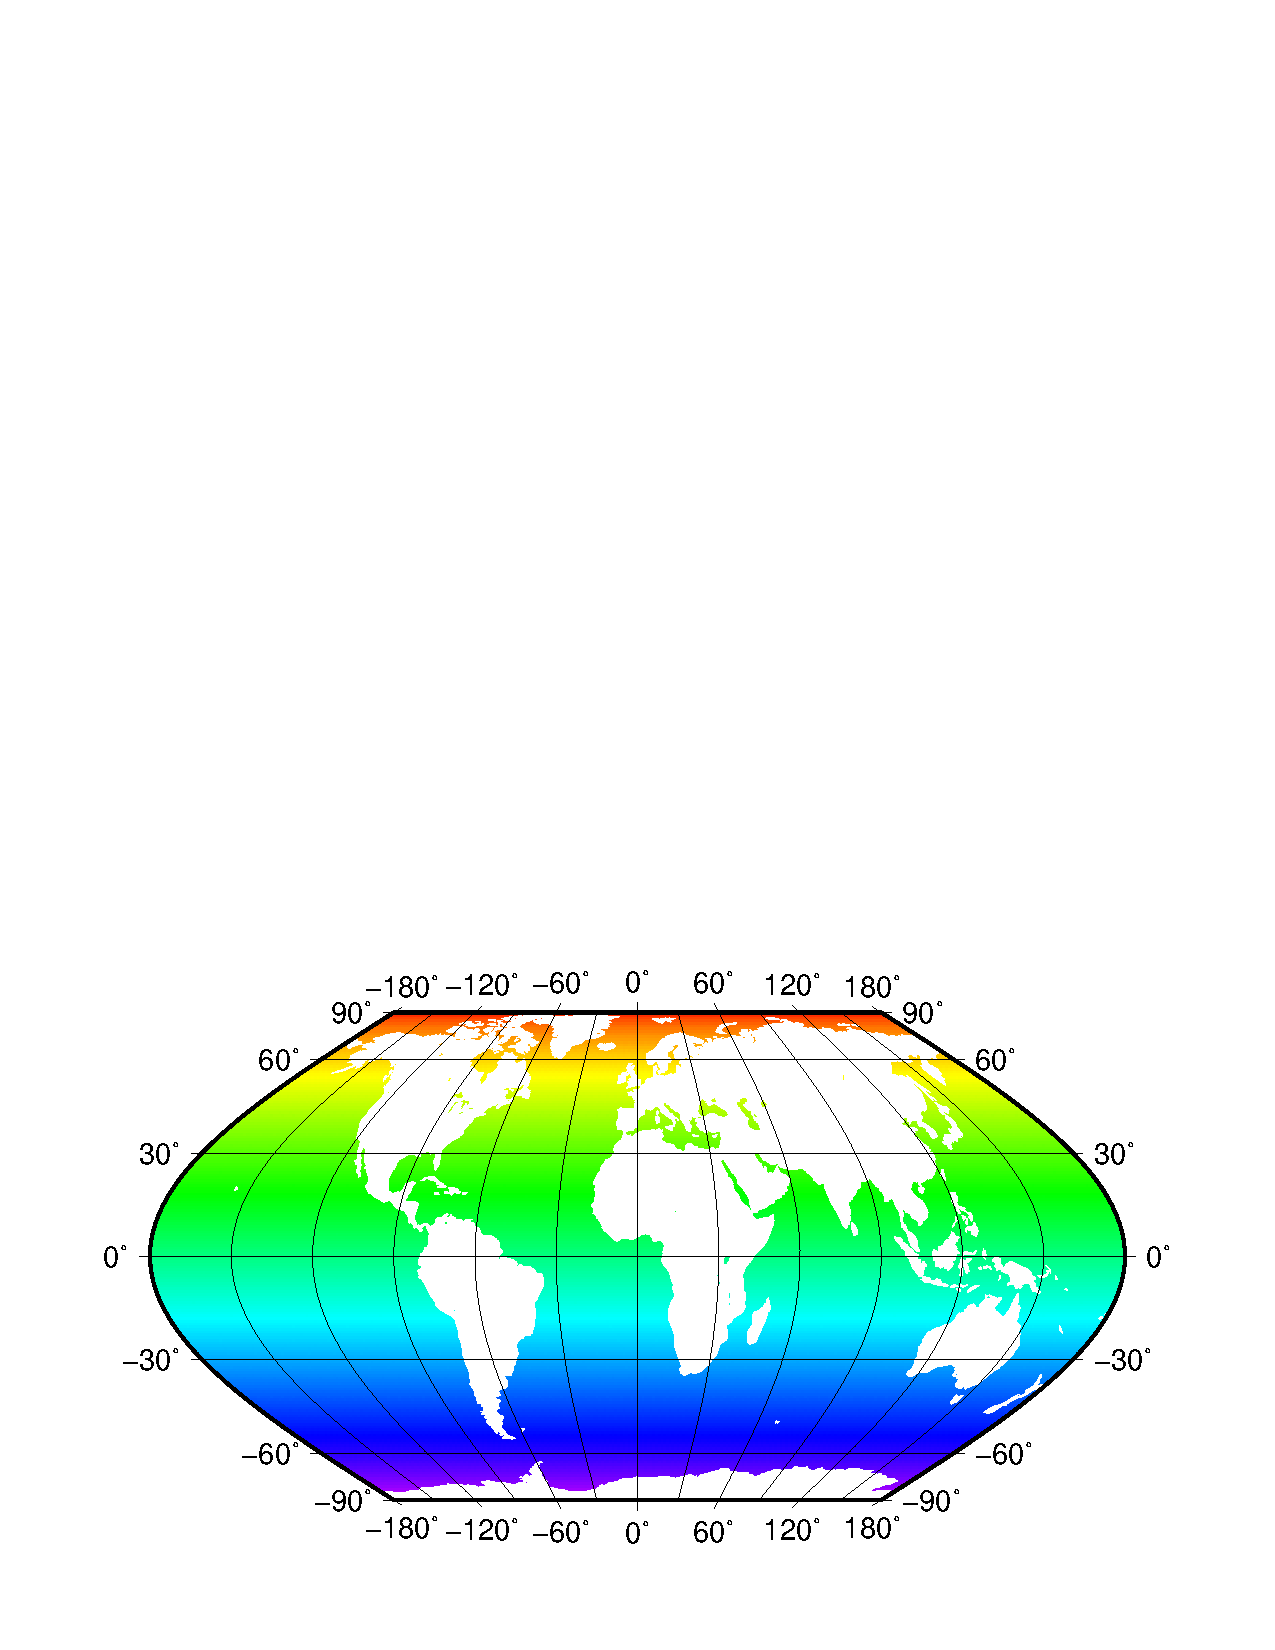
\includegraphics[width=\textwidth]{scripts/GMT_App_P_2}
\caption{Example created in isolation mode}
\label{fig:GMT_App_P_2}
\end{figure}

The files \filename{.gmtdefaults4} and \filename{.gmtcommands4} are automatically created in the temporary directory \filename{\$GMT\_TMPDIR}. The script is also adjusted such that the temporary grid file \filename{lat.grd} and colormap \filename{lat.cpt} are created in that directory as well. To make things even more easy, \GMT\ now provides a set of handy shell functions in \GMTprog{gmt\_shell\_functions.sh}: simply include that file in the script and the creation and the removal of the temporary directory is reduced to a single command.

\script{GMT_App_P_2}
\index{Isolation mode|)}

\section{Using both \gmt\ 3 and 4}
\index{\GMT, using 3 and 4}

We encourage all \GMT\ users to start using version 4 immediately; it has been tested extensively by
the \GMT\ team and has benefitted from bug reports for the 3.4.x versions.  Users who still worry about the
new version breaking things may install \GMT\ 3.4.x versions and 4.x and use our utility \progname{gmtswitch}
to select their current version should the need to switch arises.  You will find \progname{gmtswitch}
in the top-level \GMT 4.x directory; install as explained below.

Because \GMT\ 4.x is backwards compatible with the 3.4.x series yet maintains its parameters
and history in separate hidden files (e.g., \filename{.gmtdefaults4} versus \filename{.gmtdefaults})
it is possible to install and use both versions on the same workstation.  To simplify such
setups we supply the utility \progname{gmtswitch} which simplifies switching back and forth
between any number of installed \GMT\ 3-versions and \GMT\ 4.x.  Place the \progname{gmtswitch} Bourne
shell script in your
general executable path (not in one of the \GMT\ bin directories) and run it after you have
finished installing all \GMT\ versions of interest.  The first time you run \progname{gmtswitch}
it will try to find all the available versions installed on your file system.  The versions
found will be listed in the file \filename{.gmtversions} in your home directory; each line
is the full path to a \GMT\ root directory (e.g., /usr/local/GMT3.4.2).  You may
manually add or remove entries there at any time.  You are then instructed to make two
changes to your environment (the details are shell-dependent but explained by \progname{gmtswitch}):
\begin{enumerate}
\item \progname{gmtswitch} creates and maintains a symbolic link \filename{this\_gmt} in your home
directory that will point to a directory with one of the installed GMT versions.
\item Make sure {\bf \$HOME}/this\_gmt/bin is in your executable {\bf PATH}.
\end{enumerate}
Make those edits, logout, and log and back in again.  The next time you run \progname{gmtswitch}
you will be able to switch between versions.  Typing \progname{gmtswitch} with no argument will list the
available versions in a numerical menu and prompt you to choose one, whereas \progname{gmtswitch} {\it version}
will immediately switch to that version ({\it version} must be a piece of unique text making
up the full path to a version, e.g., 3.4.2).  If you use \progname{tcsh} or \progname{csh} you may have to type
``rehash'' to initiate the path changes.
